\documentclass{article}

\usepackage{float}
% \usepackage{floatrow}
\usepackage[english, serbian c]{babel}
\usepackage[utf8]{inputenc}
\usepackage[T2A]{fontenc}
\usepackage{xcolor}

\usepackage{hyperref}
\hypersetup{colorlinks,linkcolor={teal},citecolor={magenta},urlcolor={blue}}  

% \usepackage[colorlinks=true, allcolors=blue]{hyperref}

\usepackage[a4paper, total={6in, 8in}]{geometry}

% Useful packages
\usepackage{amsmath}
\usepackage{graphicx}

\title{\textbf{Дигиталне урбане мреже и друштвени медији}

\vspace{10}
\small{Семинарски рад у оквиру курса \\Рачунарство и друштво \\
        Математички факултет у Београду}}
\author{Тамара Јевтимијевић, 261/2017\\ \textit{mi17261@alas.matf.bg.ac.rs}}
\date{28. април 2022.}

\begin{document}
\maketitle

\begin{figure}[h!]
\centering

\includegraphics[width=0.25\textwidth]{slike/grb.png}
\end{figure}

\vspace{30}
\begin{abstract}
Златна грозница данашњег времена односи се на рударење података за комерцијалну употребу. У циљу зараде и комерцијализације, корпорације, које се баве информационо - комуникационим технологијама, често активно и агресивно нуде услуге на рачун опште популације. Заједно са паметним градом, концепт безбедног града је такође пример где корпорације, које се баве информационо-комуникационим технологијама, имају највише утицаја и може се рећи да је рударење података стратегија за обогаћивање тих корпорација. Крајем XX и почетком XXI века информационо - комуникационе корпорације су доживеле највећу експанзију. Данас их има све више и све су утицајније. Технологије су узнапредовале великом брзином и своје гране пустиле су свуда. Данас где год да се окренемо дигитализација је око нас. У наставку ће бити више речи о томе како је дигитализација допринела развоју градова, побољшању живота људи у градовима и како су технологије заокупирале читав свет.
\end{abstract}

\newpage
\tableofcontents

\newpage
\section{Увод}

Како се повећавају урбани изазови (саобраћај и одрживи развој града, енергетски развој града, водна инфраструктура, ...), пропагирани урбанизацијом и растом становништва, већина градова се окреће коришћењу различитих модерних технологија. Разлози за прихватање технологија су сазнање да технологије, коришћењем података генерисаних из града у ком се користе, имају потенцијал да пруже дугорочно решење, које ће утицати на ефикасност и исплативост живота у градовима. Такође већина инфраструктура и основних садржаја су дизајнирани да служе само одређеном броју људи, иако то не би требало бити случај. Ипак, као што је показао Bavel (\cite{b_2013}), у блиској прошлости, посебно крајем XX и почетком XXI века, урбане границе су се проширивале, посебно због ширења урбаних средина, а број становника у њима се повећао. Са разноликим технологијама, посебно оним које су удружене са концептом паметног града (\textit{Smart city}), повећала се могућност праћења изазова и потреба становништва. Стога су урбане структуре управљања у стању да боље разумеју количину ресурса и инфраструктуре који су потребни да би се обезбедило да градови постану уточишта за сигурност, животну способност и економски раст.

\subsection{Статистике напредовања паметних градова кроз монопол}
Успех коришћења технологија у експерименталним градовима, као што је Сонгдо у Јужној Кореји (\textit{Kolotouchkina & Seisdedos} \cite{2017}), привукла је незаситу потражњу за овим технологијама на глобалном нивоу, а такође ову потражњу је подстакао и пораст бројних фирми и компанија које се баве информационо-комуникационим технологијама. Тржиште технологија је толико уносно, јер се стално шири, развија и повећава. Извештај компаније Grand View Research (\textit{Grand View Research} \cite{2019}) проценио је тржиште паметног града на 71,3 милијарде долара у 2018. години и предвидео пораст на преко 237,6 милијарди долара до 2025. године по сложеној стопи од 18,9\%. Још један извештај Markets and Markets Inc. (\textit{Singh} \cite{s2019}) у истом периоду показује да је ово тржиште процењено на 308 милијарди долара од 2018. године и са сложеном стопом раста од 18,4\%. Та вредност би требало приближно да буде 717,2 милијарде долара до 2023. године. Различите бројке показале су како је технолошко тржиште толико експанзивно да није пронађена квантибилна метода за процену његове вредности. Ипак, заједничко у ова два извештаја је то да су паметни градови и градови са технолошком наклоношћу уносна тржишта за технолошке старт-апове. Компаније као што су IBM Corporations, Cisco Systems, Microsoft, Hitachi, Huawei, Ericsson, Schneider Electric, Accenture, Intel, Oracle и Ericssons воде у трци за главног добављача технологија. 

\subsection{Решавање проблема страних старт-апова}
За успешну примену технологија у појединим градовима неопходна је сарадња између локалних и међународних старт-апова. Ово би могло обезбедити несметани пренос знања. Веома је важно да таква сарадња осигурава да су пројекти усклађени за подршку економског раста и да обезбеђује да грађани буду циљни корисници пројеката и да их обавештавају о урбанистичким пројектима, а када је могуће и да учествују у развоју и примени пројеката. То би се могло остварити нуђењем технолошки оријентисаног посла и трансфером знања, а кроз обуку их учити како да користе податке прикупљене са личних уређаја, истовремено обезбеђујући да се пројекти поштују и подржавају.

\section{Дигитална урбана инфраструктура}
Утврђено је да је пре појаве технологија, какве данас постоје, градовима и урбаним подручјима било најбитније да успоставе чврсту инфраструктуру, јер се на то гледало као на моћно решење за урбане проблеме. Из тог разлога су већина општина и локалних влада настојале да имају најскупљу и најразвијенију инфраструктуру као што су мостови, путне мреже, аеродроми и луке. Упркос важности која се придаје овој инфраструктури, изградња инфраструктуре често је била онемогућена низом значајних изазова са којима се већина градова морала суочити. Финансијски терет је увек био један од главних изазова, стога је примећено да градови широм света имају различите нивое инфраструктурног развоја. 
\\\\
Данас већина тих чврстих инфраструктура је и даље присутна, али има потребу за надоградњом. Та надоградња је неопходна због све већег броја возила и резултујућих урбаних притисака, тако да је појам тврде инфраструктуре као решење за урбане проблеме данас поприлично застарео. Појава технологија, које омогућавају коришћење података за решавање већине урбаних изазова, нуди извесно олакшање финансијских ограничења са којима се суочава већина градова. На пример у случају Шангаја (Слика \ref{fig:sangaj}) ефикаснија употреба возила и кретања може бити обезбеђена помоћу технологија. Појава технологија подстакла је градове да траже ИКТ оријентисане компаније, које би могле да обезбеде технологије, које ће да дају корисне податке у решавању елементарних проблема. \\
\begin{figure}[h!]
\centering
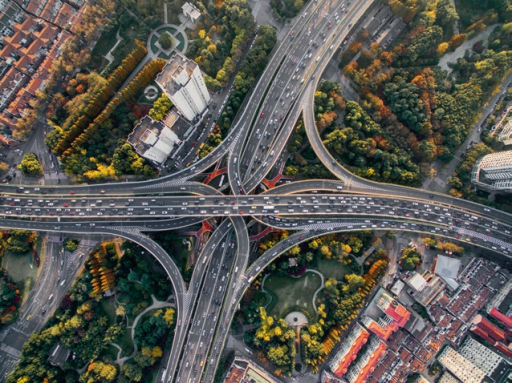
\includegraphics[width=0.6\textwidth]{slike/sangajska_petlja.png}
\caption{\label{fig:sangaj}Шангајска петља, која приказује сложени инжењеринг и инвестиције потребне у чврстој инфраструктури}
\end{figure} \\
Међутим, кроз дигиталне технологије те тврде инфраструктуре, које се сматрају неефикасним у решавању урбаних изазова, добијају нове вредности. Неке од њих се реновирају и регенеришу да би се поново користиле за различите сврхе, а не за њихове првобитне. Тврда инфраструктура има користи од урбаних дигиталних решења, посебно у погледу оптимизације коришћења ресурса током конструкција. \\\\
Са новим технологијама примећено је да нове грађевинске компаније користе материјале и ресурсе који су одрживији, издржљивији и пружају минималан утицај на животну средину. Такође користе и оне материјале који имају потенцијал да издрже различите изазове, као што су екстремни временски услови (на пример превише ниска или превише висока температура). Присуство дигиталне технологије у урбаним срединама омогућило је мере усмерене ка ублажавању емисија штетних гасова, посебно наглашавањем ниске потрошње енергије у зградама, транспортним мрежама и другим инфраструктурама. Дигиталне технологије су такође отвориле нове платформе за поновну употребу и рециклажу материјала, чиме се помаже у смањењу емисија штетних гасова, као и у заштити животне средине од штетних материјала, који у већини случајева нису биоразградиви и садрже елементе који имају потенцијал да загаде и угрозе интегритет подручја и живот људи. \\\\
Урбана дигитална решења гарантују нове трендове из којих потиче то да инфраструктурни развој више не контролишу само компаније које су се бавиле изградњом тешке инфраструктуре, већ и ИКТ провајдери. Појава дигиталних технологија градовима пружа додатну вредност, јер се помоћу њих повећава потенцијал за решавање урбаних изазова, док се истовремено постиже и одрживост, отпорност, економски раст као и услови за живот по приступачној цени. 
% \newpage
\section{Успон информационо - комуникационих технологија}
Информационе технологије су научна дисциплина, која се јавља крајем двадесетог века, са преласком друштва из индустријског у информатичко доба. Од тад па све до данас изузетно се брзо развија и шири њихова употреба са непрекидним појављивањем нових технологија. Имају огроман утицај на људско друштво у свим аспектима. Информационе технологије користе рачунаре и рачунарске програме за безбедну конверзију, складиштење, заштиту, обраду, пренос и претраживање информација.
\\\\
Термин информационе технологије често обухвата и знатно шире поље области технологије. Све оне активности којима се ИТ професионалци баве, од инсталације апликативних програма до пројектовања сложених рачунарских система. Неке од тих активности су: умрежавање и инжењеринг рачунарског хардвера, дизајнирање софтвера и база података, као и управљање и администрација информационим системом. Термин информационе технологије први је употребио Џим Домсик из Мичигена, новембра 1981. године. \\
У последње време термин информационе технологије се проширује да се нагласи употреба комуникација, посебно електронских. Информационо - комуникационе технологије обухватају технологије као што су стони и преносни рачунари, софтвер, периферни уређаји и уређаји за повезивање на Интернет који су намењени за обраду информација и комуникацију.\\\\
Најважнију компоненту информационо - комуникационих технологија представљају рачунари. У исто време, применом и развојем дигиталних комуникација омогућен је лак, брз, ефикасан и јефтин начина размене информација. ИКТ имају фундаменталан утицај на модерно друштво јер начини размене и преноса, као и количина најразличитијих информација данас су већи него икада пре у историји. Данас пословне организације користе ИКТ за побољшање квалитета производа и услуга, повећање продуктивности рада, уштеду енергије и новца и на крају за повећање профита. \\\\\\\\
Дакле, информационо - комуникационе технологије су током само једне људске генерације револуционарно промениле начин живота, учења, рада и забаве. ИКТ све дубље трансформишу начин интеракције људи, предузећа и јавних институција. Укупне промене у свим аспектима друштва које су омогућене применом ИКТ чине развој информационог друштва. Успешан развој информационог друштва захтева одговарајући степен знања и вештина, како код стручњака разних професија, тако и код осталих грађана. Поред повећања потребе за вештинама у вези примене ИКТ, Интернет је променио начин ширења знања и информација у свим областима.

\subsection{Монопол ИКТ-а}
Распрострањеност и популарност урбаних дигиталних решења се повећала појавом технологије података. Та распростањеност и популарност је постигнута због доступности уређаја и компоненти, које имају могућност хватања различитих облика података. Велика распрострањеност паметних телефона помаже у генерисању значајних количина података, а када се ти подаци комбинују и анализирају чине снажно оруђе, које има потенцијал да информише и обликује активност у градовима. Потенцијал информационих технологија тј. паметних телефона је инспирисао нова пословна решења, која су корпорације и пионирски старт-апови прихватили и капитализовали, да би стекли конкурентску предност на тржишту пружања ИКТ решења. Флорида (\cite{florida_2018}) показује како је ова доступност помогла у стварању успешних предузећа као што су Uber, Airbnb, Didi Chuxing, WeWork, Lyft, Mobike и Delivery Hero. Уз то су, може се рећи, и конкуренти водећим компанијама као што су Apple, Alphabet, Facebook, Amazon, Alibaba, и другим сличним, које су формирале своје корене ослањајући се на "\textit{paper of technology}", и још више, ослањајући се на доступност података. Извештај ЕY (\cite{ey_2014}) подржава аргумент да је доступност података сада видљива као основна конкуренција, посебно у приказивању реалног времена. Извештај показује да су најуспешније компаније оне које имају доступне податке или ће управљати, инвестирати, хватати, чувати, агрегирати, анализирати и извући вредност из доступних података.
\\\\
Слично налазима из извештаја ЕY, Singh (\cite{s_2019}) је обавио истраживање о акумулацији богатства, којим је показао да дигиталне компаније расту и узнапредују доста брже у односу на њихове традиционалне колеге. Аутор приписује овај раст повећању заинтересованости градова широм света да обезбеде дигитална урбана решења, чиме се дигитално тржиште чини уносним са трилионима долара.  Опсежна анализа Govindarajan, Rajgopal и Srivastava (\cite{g_r_s_2018}) показује да се у савременом свету одлуке о инвестицијама компанија руководе вредношћу поврата обима на нематеријална улагања, а не традиционалним фокусом. Ову тврдњу су поткрепили наводећи примере попут куповине WhatsApp-а од стране Facebook-а по цени од 19 милијарди долара упркос томе што WhatsApp нема пријављених финансијских извештаја. Слично томе, аутори наводе случај Twitter-а који је успео да уђе у иницијалну јавну понуду са процењеном вредношћу од 24 милијарде долара, упркос извештајима да је направио губитак од 79 милиона долара пре ове планиране иницијалне јавне понуде. Они су показали да су ове дигиталне компаније у стању да преброде негативну ознаку опадања биланса кроз своју способност да наставе да користе дигиталне платформе, које имају неограничене могућности. Према њима финансијски извештаји, у већини случајева, дају другачију слику о реалном стању компаније.
\\\\\\\\\\
Напредак дигиталних компанија може се делимично приписати њиховој решености да значајно уложе своје време, труд и ресурсе у истраживање и развој. Одлуке о улагању у истраживање и развој подстакнуте су повећањем конкуренције како малих, тако и великих компанија, које се баве обезбеђивањем дигиталних решења. Треба напоменути и то да постоји значајан број искусних компанија, које пружају информационо-комуникационе технологије. Да би се такмичили са њима, како саветује Влада Квинсленда (\cite{q_2016}), старт-апови морају да преусмере своје напоре ка областима као што су истраживање тржишта, како би се упознали са стварним локалним питањима и захтевима, које свако циљно тржиште настоји да задовољи. Како су објаснили Karvonen и van Heur (\cite{v_h_2014}) дигитална решења нису класична тј. конвенционална, као она која могу да се копирају и пренесу из једног града у други, баш због различитих захтева сваког града. На пример, у сектору транспорта, Uber и Lyft, иако раде у истом географском региону и циљају на сличне базе купаца, су технички различити, а такође се разликују и у смислу тржишне вредности. Међутим, они деле сличне дигиталне и технолошке платформе. Yu, Liu, Fung и Leung  (\cite{l_2018}) објашњавају да су такве разлике подстакнуте нивоом улагања у истраживање и развој од стране различитих компанија. Дакле, њихова величина и вредност не могу бити исти. Ту истину потврђују Han, Tomas, Yang, Leromonachou и Zhang (\cite{zhang_2017}), који су приказали да највиша технологија индустрије можда неће имати користи од истраживања и развоја ако стратегије, које се користе за комерцијализују дигиталних решења, које компаније користе, нису ефикасне. То је случај код већине кинеских компанија које су посматране.
\\\\
Обимно улагање у истраживање и развој дигиталних технологија ће на крају фаворизовати развој власничких технологија, које се промовишу тако да осигурају економски просперитет градова, посебно напомињући да су такви градови скројени за решавање локалних захтева и изазова. Стога, као што се у великој мери говори у извештају McKinsey (\textit{McKinsey \& Company} \cite{mc_2018a}), већина градова се одлучује за партнерство са добављачима решења, који им гарантују да њихова дигитална решења имају капацитет да се суоче са локалним изазовима града. На пример, Taylor (\cite{t_2014}) је приметио да већина ИКТ корпорација сада унапређује и усавршава концепт паметних градова и каже се да су информационо - комуникациону технологију означили као ону која има одговоре на све урбане изазове. Поред технологије '\textit{Smart city}', за решавање урбаних изазова помогли су и истраживање и развој старт-апова, попут Твитера и Фејсбука, који су урбаном дигиталном тржишту дели решења кроз велике податке, које контролишу од великог броја корисника ових платформи.
\newpage
\section{Друштвене мреже и град}
Успон друштвених мрежа као што су Facebook, Тwitter, WeChat, Tumblr, Instagram, Google+, YouTube, Linkedin, TikTok, Snapchat и WhatsApp такође је променио начин на који људи широм света комуницирају и живе (Слика \ref{fig:mreze}). Чини се да људи више воле и примењују дигиталне интеракције у односу на физичке интеракције. Према Tjepkema (\cite{t_2019}), процењује се да преко 3,2 милијарде људи широм света користите друштвене мреже на овај или онај начин, а ови трендови су заслужни за широк продор паметних уређаја као што су мобилни телефони и таблети. Способности ових уређаја да подрже различите апликације друштвених мрежа чине да ширење и повезаност буду још експанзивнији и чини да утицај друштвених мрежа на људе буде још јачи. Што се тиче утицаја на живот људи, неки тврде да су друштвене мреже имале броје позитивне утицаје на људе и њихов живот, међутим значајан број других мисли другачије. Већи је број оних који сматрају да су друштвене мреже донеле много више негативног,  него позитивног. О утицају друштвених мрежа на живот људи истраживали су  Hemsley, Jacobson, Gruzd и Mai (\cite{m_2018}), како би се утврдило да ли су друштвене мреже донеле више добра или зла. Утврдили су да то зависи само и искључиво од појединаца и њиховог искуства са друштвеним мрежама. Ипак, они истичу да су друштвене мреже итекако имале свој утицај у областима попут управљања, економског раста, безбедности, образовања, здравственог и транспортног сектора и у још многим другим сферама и областима. Слично, они такође показују да како је ширење друштвених мрежа постало све веће, долази до случајева кршења приватности, лажних вести, терористичких активности као што су регрутовање, сајбер насиља, интернет превара, крађе идентитета, зависности од интернета и друштвених мрежа, моралне декаденције и још многих других лоших ствари. \\
\begin{figure}[h!]
\centering
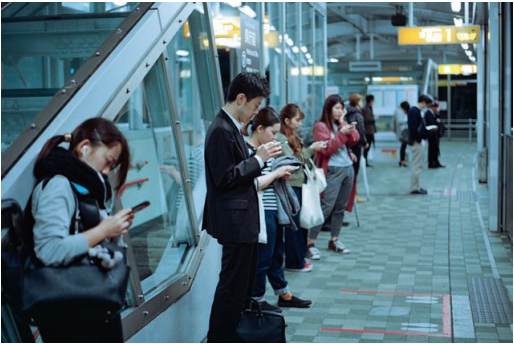
\includegraphics[width=0.6\textwidth]{slike/drustvene_mreze.png}
\caption{\label{fig:mreze}Људи на својим телефонима док чекају метро у Нахи, Јапан}
\end{figure}
\\\\
У политичкој сфери постојале су различите платформе друштвених мрежа, које су се користиле као алат за кампању са противницима. Кроз платформе политичари су у могућности да дођу до мноштва својих присталица у реалном времену путем текста (реклама), видеа или стрима уживо. На тај начин омогућавали су да њихове присталице учествују у дискусијама и ћаскањима уживо. 
\\\\
Исте платформе користе политички противници да дискредитују једни друге, а у најгорем случају, поменуте платформе коришћене су у неким земљама за обарање влада, па чак и за преокрет избора. Tufekci (\cite{tu_2014}) објашњава како су у Египту друштвене мреже биле главно средство у организовању устанка и револуције која је довела до тога да је председник Хосни Мубарак свргнут са своје функције. Saifuzzaman (\cite{s_2017}) говори о томе како су у сиријским немирима млади демонстантни виђани на улицама са паметним телефонима у рукама, вероватно ослањајући се на различите облике ажурирања путем различитих друштвених мрежа за различите старосне групе и за глобалну публику. Ово је приказ лошег удела друштвених мрежа у свету, јер данас је веома лако ширити све, па и мржњу и незадовољство, преко друштвених мрежа. На жалост та предност може бити погубна, као што је било у случају Египта. Данас млади преко друштвених мрежа најлакше деле све међусобно, јер се на такав начин избегава безбедносна цензура. То се посебно односи на младе демонстранте широм света, јер им друштвене мреже и избегавање безбедносне цензуре даје предност у логистици и пружа им већу пажњу јавности.
\\\\
Спој урбаног отвореног простора и друштвених мрежа је феномен виђен и у недавним политичким манифестацијама у различитим деловима света. Протести и догађаји су често повезани са употребом дигиталних медија и друштвених мрежа. Убрзано коришћење мобилних телефона и сцене као на слици \ref{fig:mreze2} сматрају се уобичајеним и можда чак и најпогоднијим начином за прикупљање и пренос података у тим околностима.\\
\begin{figure}[h!]
\centering

\includegraphics[width=0.6\textwidth]{slike/mreze2.png}
\caption{\label{fig:mreze2}Коришћење мобилних телефона за снимање политичких манифестација}
\end{figure}
\\\\
Schwedler (\cite{s_2013}) објашњава да доступност отворених јавних простора даје подстицај грађанским и политичким активностима због њиховог капацитета и локације. Low (\cite{l_2017}) истиче да су ове карактеристике отворених простора биле кључне у катализацији бурних догађаја попут Арапског пролећа, посебно у Египту, Тунису и Турској. Такође, били су кључни у ономе што је познато као „глобални покрет окупације“ са примерима као што су Окупирај Бостон, Окупирај Волстрит и Покрет Жутих прслука у Француској. У основи ових догађаја на јавним местима се види коришћење друштвених мрежа као платформе за комуникација и подстицање. \\\\\\
Још један практичан пример коришћења урбаног отвореног простора за политичке манифестације, како објашњавају Chrona и Bee (\cite{cb_2017}), је случај покрета Окупирај Гези у Турској. Речено је да се хетерогена мешавина демонстраната, који представљају мешавину грађана, организовала путем друштвених мрежа и договорила да се окупе у парку Гези како би испољили своју фрустрацију због ауторитарног режима. Путем друштвених мрежа, посебно преко Фејсбука и Твитера, ажурирања у реалном времену из парка Гези су била дељена локалној и међународној публици и то је учинило да се број демонстраната повећава сваким даном све више и више. Протести нису само постигли политичке циљеве, већ су и помогли да се очува парк, који је локална власт планирала да сруши и да ту изгради тржни центар и џамију (Kuymulu, \cite{k_2013}).
\\\\
Улога друштвених мрежа у градовима превазилази политику и утиче и на друге области као што су друштвени живот, одрживост, туризам, бизнис, инфраструктурни развој и још многе друге. На пример, на одлуку код људи, везано за путовања, у великој мери утиче оно што људи виде на друштвеним мрежама, одатле потичу и велики и енергични напори градова да улажу у брендирање и маркетинг са циљем да постану привлачни путницима, који доносе економске прилике. За реализацију свега тога захтевају се нови приступи као што су урбана регенерација, улагање у нову инфраструктуру, усвајање одрживих стратегија које би очистиле град од свих врста загађења. Такође потребно је усвојити и технологије за побољшање животних услова, сигурности и отпорности. Такође, захтева се и усклађена сарадња између различитих заинтересованих страна и активно учешће грађана. Дакле, промена у перцепцији и омогућавање да се поседују пројекти као што су на пример #IAmsterdam и #magicalKenya, што добро одјекује и код становника и код посетилаца. Јасно је да је развој друштвених мрежа значајно утицао на урбана подручја и на развој урбаних подручја.
\\
\newpage
\section{Урбано брендирање и друштвене мреже}
Појава дигиталних решења, која се фокусирају на градове и урбана подручја је имала бројне позитивне стране као што је могућност брендирања града. Дигитални бренд је дао градовима прилику да дигиталне технологије искористе на економској граници, као што је урбани туризам, где се промовише инфраструктура и привлаче посетиоци, како домаћи тако и страни. Фокус на урбани туризам је подстакнут сазнањем да би у будућности требало да већина становништва живи у градовима, а само мали број њих ће остајати на селу. По инстраживању то ће се повећати са садашњих 54\% на преко 68\% до 2050. (United Nations, \cite{un_2017}). Поред тога што градови привлаче велики број људи који желе да живе у њима тј. поред стамбене компоненте, примећено је и да привлаче велики број оних који их посећују због посла и разоноде. Такође се примећује да градски превоз, тј. градска путовања чине преко 45\% глобалних међународних путовања (Светски савет за путовања и туризам, \cite{wt_2018}). World Travel \& Tourism Council (\cite{wt_2018}) показује како таква путовања утичу и на иновације градова тј. промене у градовима, јер сваки покушава да победи у борби за посетиоце. Novelli (\cite{no_2005}) објашњава како су такве иновације довеле до брендова као што су здравствени и стоматолошки туризам, образовни туризам, туристички и рекреативни туризам, пословни туризам, културни и уметнички туризам и још многи други.
\\\\
Након појаве друштвених мрежа тј. медија, такви туристички брендови су прихваћени у различитим градовима кроз стратегије прилагођене различитим корисницима на различитим платформама друштвених мрежа (Almeyda-Ibáñez \& George \cite{ag_2017}; Kerr, Dombkins \& Jelley \cite{kdj_2012}; Pike \& Page \cite{pp_2014}).
На пример, Амстердам, уметнички град са култним музејима и богатом историјом, усвојио је израз „ЈА АМСТЕРДАМ“, приказан на  знаку који носи ту фразу и налази се испед музеја Rijksmuseum, као што је приказано у Слика \ref{fig:amsterdam}. 

\begin{figure}[h!]
\centering

\includegraphics[width=0.6\textwidth]{slike/amsterdam.png}
\caption{\label{fig:amsterdam}Брендирање у Амстердаму}
\end{figure}\\
Према Hitti (\cite{hitti_2018}), знак има велику моћ привлачења туриста у град. Његова популарност је дошла захваљујући Твитер хештегу „#IAmsterdam“, који га је промовисао до те мере да га је приметио велики број људи и да је да је преко 6000 селфија снимљено испред њега сваког дана и већина њих је подељена путем Твитера (Newberry, \cite{nb_2016}). \\\\
Брендирање је стратегија која је усвојена, да би се они, који су у овом случају живели у Аместердаму и у њему радили, али и они који су га само посетили осетили његовим делом. Брендирање је у случају Амстердама имало огроман утицај које је резултовао тиме да је град увек био пренасељен до тачке да је тема туризма постала контрапродуктивна. У једном тенутку је градско руководство одлучило да склони знак "IAMSTERDAM", међутим склањање знака није био добар потез, критикован је од стране локалног становништва које је користило хештег #IAmsterdam. Упркос томе што су слова уклоњена, Hitti (\cite{hitti_2018}) тврди да "IAmsterdam" стратегија брендирања има неизбрисив траг на туристичкој ознаци града Амстердама, а чак ни уклањање знака не може избрисати успех који град постиже. Овде је наведен само пример Амстердама, оваквих примера брендирања града има много и то је у данашње време постало веома популарно.
\\\\
Други градови, као што су Измир, Истанбул, Лион, Чикаго, Сингапур, Берлин, Данди и бројни други, прилагодили су своје стратегије брендирања на друштвеним мрежама. У Дандију, на пример, брендирање је почело још 2011. Почело је тако што је град направио промоцију под слоганом 'Освоји викенд у Дандију' циљајући на младо становништво које живи чак и изван града. До данас град одржава активно присуство на друштвеним мрежама под слоганом „Dundee: One City, Many Discoveries“ (Dundee: Један град, много открића), а  та промоција је била кључна у његовом брендирању. Што се тиче брендирања Измира, Saatçioğlu (\cite{sa_2017}) каже да се град Измир промовисао путем друштвених мрежа тако што су се на Инстаграму и Фејсбуку приказивале фотографије под називом „Места које треба видети“ , а то је имало позитиван утицај на промоцију града. Други градови, како су објаснили Higham и Moyle (\cite{hm_2016}), капитализовали су спортску културу града и брендирали се као центри за спортски туризам. На пример град Ливерпул, који је дом фудбалског клуба Ливерпул, искористио је популарност овог тима да своју економију обликује као спортску и то су у великој мери користили за развој инфраструктуре. Такође, град је добијао огромне приходе од локалне подршке и подршке на даљину, који посећују град због фудбала и спортских активности.
\\\\
Да би се одржао темпо дигиталног брендирања, примећује се да се већина градова определила да регрутују младе и технолошки потковане и способне људе, чији је задатак да предводе и развијају нове облике комуникација и технологија. Holt (\cite{ho_2016}) објашњава да је то важно јер друштвене мреже имају потенцијал да поремете културни идентитет града, па стога особље које разуме нови алат за брендирање има потенцијал да привуче млађи слој друштва, који се све више приклања новом облику културе, познатом као култура гомиле, која обухвата огроман број људи који деле слично интересовање. То укључује странице обожавалаца на Фејсбуку, а на Твитеру оне напредују под одређеним хештегом. Утицај и резултат таквог посвећеног тима за вођење иницијативе урбаног брендирања је повећан број посетилаца, који су спремни да користе услуге које град нуди. Rehan (\cite{re_2014}) објашњава, да урбани бренд промовише концепт одрживости и служи као комуникациони алат, који омогућава градовима да се пласирају на тржиште. 
\\\\
За инвестиције се каже да стварају комплекс и боље искуство мрежа, које обухватају секторе као што су угоститељство, излети и путовања, транспорт, финансијски сектор и сектори урбаног управљања и још многе друге. Имати такве секторе на истој платформи тј. друштвеној мрежи помаже у смањењу јаза између креатора политике, урбаног менаџмента, приватног сектора и грађана, а то омогућава сарадњу у формулисању политика, које помажу да се побољшају сектори, а на крају и економски статус града.

\section{Закључак}
Можемо приметити све већу улогу дигиталних медија у
обликовању градске привреде и политичке сфере. Улога друштвених медија, односно мрежа у градовима, посебно у јавним просторима, постаје све више наглашена. Види се да политичари све више користе друштвене платформе, како би стекли политичку километражу и економску отпорност кроз повећање активности у вези са туризмом, коришћењем нових, технолошки прилагођених техника брендирања и маркетинга.

\newpage
\bibliographystyle{unsrt}
\bibliography{bibliography} 

\vspace{-7}
\bibitem{} [35] Zaheer Allam. Cities and the  Digital  Revolution Aligning technology and humanity. \emph{Digital Urban Networks and Social Media}: 61-83. \\

\vspace{-10}
\bibitem{} [36] \href{http://miticmirjana.weebly.com/104810501058-10901077109310851086108310861075108011121077.html}{Informaciono-komunikacione tehnologije}

\end{document}